\documentclass[11pt,a4paper]{article}
\usepackage[utf8x]{inputenc}
\usepackage{ucs}
\usepackage{amsmath}
\usepackage{amsfonts}
\usepackage{amssymb}
\usepackage{fancyvrb}
\usepackage{url}
\usepackage{graphicx}
\usepackage{subfigure}

\author{HU, Pili and LI, Yichao}
\title{Community Detection on 2-Hop Topology}

\newcommand{\question}{\textbf{---NEED-REVIEW-HERE---}}

\begin{document}

\maketitle

\begin{abstract}
	Community detection in social networks has drawn great interest
	in recent decades, especially inspired by the emerge of wide 
	online social network sites. In this paper, we study the two-hop 
	topology from several observers in the "renren.com" network. 
	Some important statistics are calculated first, along with 
	some visualization. Then we extract 9 features from the 
	2-hop topology. All features are evaluated alone using ROC first. 
	Then we train multiple MLP models under different settings. 
	
	The most effective features in our study is PageRank with escape
	vector to several in-community high degree nodes. 
	By eliminating leaf nodes(degree=1), we can get a prediction
	precision 0.699 and recall 0.534. The confusion matrix shows 
	this result is not trivial. 

	This document serves as the report of CSCI5180 course 
	project\cite{csci5180_lecture,csci5180_tutorial}. 
	For more information, codes, and data, please refer to 
	our open source repository\cite{hu2011-cd2hop}. 
	
\end{abstract}

\pagebreak
\tableofcontents
\pagebreak

\section{Introduction}

\subsection{Motivation}

Community detection has drawn great interest in the near decade. 
The explosion of online Social Network Sites make the study more 
practical but challenging. Traditional methodology aims at 
optimizing certain global metric. The resultant graph partition 
can thus be regarded as communities. The motivation of detecting 
communities on 2-hop topology comes in two folds: 
\begin{enumerate}
	\item \textbf{Data Availability}. The global topology of 
	those SNS is kept confidential. However, users are allowed 
	to view their buddies profile by default. This gives us the 
	chance to construct a 2-hop subgraph from the whole graph. 
	Take a step further, outsiders can always observe some forwarding 
	sequences of tweet/status. This helps to reconstruct a 
	subgraph more than 2-hop from the observer. The methodology 
	developed here can thus be extended to such situations. 
	\item \textbf{Computation Availability}. Although those SNS 
	providers have access to the global topology, it is computationally
	intractable to perform some well-developed global optimization. 
	Local heuristics are widely used in many applications. 
\end{enumerate}

\subsection{Application}

The potential application may be:
\begin{enumerate}
	\item \textbf{Friend recommendation}. This is one of the 
	most important applications of SNS. Traditional ways
	try to gather other information first, like school, company, etc. 
	Then the program recommends friends based on this information.  
	\item \textbf{Targeted advertisement}. Wide-sense community 
	can represent a group of people sharing the same interests. Their
	consumption pattern may be similar. Detecting such "communities"
	in the context where nodes are not directly labeled(like forums, 
	microblogs, etc) help social media advertisers to improve 
	their lifting ratio. 
\end{enumerate}

\subsection{Contribution}

The contribution comes in three folds:
\begin{enumerate}
	\item Output a crawler specialized for "renren.com". 
	\item Extract 9 proximity measures from 2-hop topology. 
	Those meta tools can work on 200,000 edges in the order 
	of seconds. They can facilitate future study. 
	\item Train several Multi-Layer Perceptron(MLP)s to 
	combine those proximity measures. 
\end{enumerate}

Data limitation(only 2-hop topology without content information)
distinguishes our work from previous work. This is also 
the most challenging part in our study. 

\subsection{Problem Definition}

Given one observer node in an SNS network, and 
all nodes within 2-hop from the observer, together 
with the links, try to predict whether a node is 
in the same community with the observer. If so, 
the class label is set to 1, otherwise 0. 

\section{Data Preparation and Preprocessing}

\subsection{Data Source}

The data source used in this paper is "renren.com", which is the 
most popular SNS in mainland China. At the mean while, "renren.com" 
has the following good characteristics:
\begin{itemize}
	\item Web UI of "3g.renren.com" is very clean. Cawling through
	this interface doesn't require any API calls.  
	\item Renren is a real name dense graph connected mainly through 
	real communities. Intuitively speaking, 
	people who are close to the observer should be observed within 
	this 2-hop topology with high probability. 
	\item Institution label for all nodes in the observed subgraph
	is available on "renren.com". It makes model validation easier
	and automated. If the model is proven effective, we can adapt 
	it to other SNS's, where institution label may be not available.  
\end{itemize}

\subsection{Crawler}

The crawler is developed using the following components:
\begin{itemize}
	\item \begin{verbatim}
		perl
	\end{verbatim}
	\item \begin{verbatim}
		wget
	\end{verbatim}
	\item \begin{verbatim}
		bash
	\end{verbatim}
\end{itemize}

We fake HTTP login and page requests like an ordinary user. 
Random delay between two adjacent requests is introduced 
to mitigate the automation pattern. 

For more details, interested readers are recommended to 
our project \cite{hu2011-cd2hop}. The crawler is under 
directory 'crawler', together with detailed instructions 
on how to deploy one yourself. 

\subsection{Preprocessing}

The preprocessing steps is as follows:
\begin{enumerate}
	\item Parse crawled web pages to get user ID and institution name. 
	\item Create one vertex for each person crawled. 
	\item Create one edge for each friend relationship. 
	\item Do isomorphic tranformation on the original graph
	\cite{wiki_iso_graph}. Vertex number and insitution label 
	is shuffled according to a psudorandom sequence. 
	This is to protect privacy of our volunteer observers. 
\end{enumerate}

After preprocessing, we get the raw data, which is in the
following format:
\begin{Verbatim}
---'link'---
NodeID1 '\t' NodeID2
NodeID1 '\t' NodeID3
...

---'node'---
NodeID1 '\t' Label1
NodeID2 '\t' Label2
...
\end{Verbatim}

To facilitate our model training and evaluation, 
we divide our data into two parts randomly and equally: 
one training set and one testing set. 

\section{Statistics}

Basic statistics are shown in table(\ref{tbl:stat_basic}). 

\begin{table}[htb]
\caption{Basic Statistics}
\label{tbl:stat_basic}
\begin{tabular}{c|ccc}
\hline
Observer Seq. & \# of All Nodes & \# of Level 1 Nodes & \# of Links \\
\hline
1 & 52595 & 357 & 83820 \\
2 & 88238 & 446 & 139224 \\
3 & 129019 & 535 & 204006 \\
4 & 46049 & 224 & 75654 \\
5 & 48258 & 260 & 85479 \\
6 & 22060 & 120 & 29860 \\
7 & 43086 & 181 & 60719 \\
8 & 175237 & 733 & 367785 \\
\hline
\end{tabular}
\end{table}

The number of nodes, number of level 1 nodes, and number of links
are positive related.

We plot observer2's nodes whose degree is greater than or equal to 5. 
fig(\ref{fig:o2_degree}) shows the degree v.s. rank in log log scale. 
We can see that the curve is not a linear line, as appears 
in most Zipf like distribution scenario. The curve is 
super linear, which means it is more skewed. This makes
sense because we only have 2-hop topology from the observer. 
Most edges of level 2 nodes are not present in our data. 

\begin{figure}
	\centering
	\includegraphics[width=0.6\textwidth]{fig/o2_degree_geq5.jpg}
	\caption{Observer2, Degree Distribution}
	\label{fig:o2_degree}
\end{figure}

\section{Topology Visualization}

In this study, we use NodeXL \cite{nodexl} to visualize our graph. 

NodeXL is an open source Excel plugin. Though it is easy to use, 
the process ability is not high enough for our large graph(10w order 
of nodes and 20w order of edges). We do the following 
pre-processing to make NodeXL work:
\begin{enumerate}
	\item Eliminate leaf nodes, whose degree is 1. 
	\item Sample edges in the rest graph. 
\end{enumerate}
Note that "renren.com" is a dense graph. A typical node will have 
more than 100 edges. This makes NodeXL hard to work. With random
sampling, the topology can be visualized by NodeXL. fig(\ref{fig:topo_vis})
shows the result. 

\begin{figure}
	\centering
	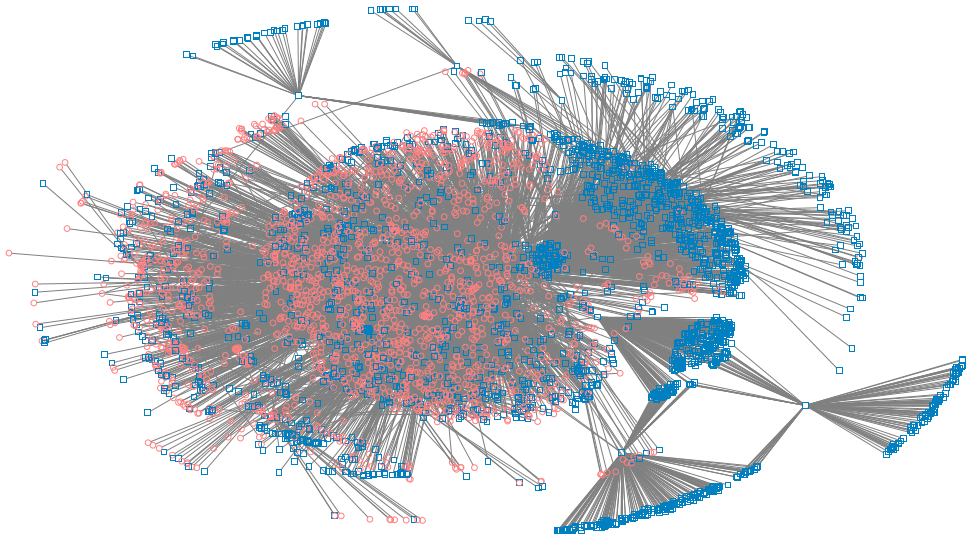
\includegraphics[width=0.8\textwidth]{../visualization/sample1W_3.png}
	\caption{Topology Visualization}
	\label{fig:topo_vis}
\end{figure}

\section{Notations}

The notations used throughout this paper are gathered 
in table(\ref{tbl:notation}). 

\begin{table}[htb]
	\centering
	\caption{Notations}
	\label{tbl:notation}
	\begin{tabular}{c|c}
	\hline
	Symbol & Explanation \\
	\hline
	$n$ & node number \\
	$m$ & edge number \\
	$A$ & adjacency matrix \\
	$A_{ij}$ & 1 if node $i$ and node $j$ are directly \\
	& connected, 0 otherwise\\
	$N(i)$ & neighbourhood of $i$, namely \\
	& $N(i) = \{j | A_{ij} = 1 \}$ \\
	$d(i)$ & degree of node $i$ \\
	& $d(i) = \sum_{j}{A_{ij}}$ \\
	$o$ & observer \\
	$\overrightarrow{v}$ & ranking vector of nodes \\
	$l_i$ & the real label of node $i$ \\
	$L_i$ & the predicted label of node $i$ \\
	\hline
	\end{tabular}
\end{table}


\section{Feature Selection}

\subsection{Random Walk Based Techniques}
\label{sec:prox_pr}

The rationale behind random walk is: the nearer a node
is to observer, it can be reached with a higher probability by a random 
	walker starting from observer. PageRank is one of the most classical work 
	in this field.

We shortlist three variations\cite{aggarwal2011social} of the original 
PageRank, together with the explanation of using them in our context:
		\begin{itemize}
			\item PageRank with escape probability:
			\begin{equation}
				\overrightarrow{v} = \alpha A^{\rm T}\overrightarrow{v}
				+ (1-\alpha)\frac{\overrightarrow{1}}{n}
				\label{eq:pr}
			\end{equation}
			where $A$ is the transition matrix, typically the adjacency matrix,
			and $\alpha$ is the transfer ratio. $ \overrightarrow{v} $ is 
			the resultant PageRank value. 
			
			In our graph, the link is very sparse for edge node, which 
			represents the friend of observer's friend. They provide 
			many dangling links, which influences the outcome of 
			original PageRank algorithm. These nodes may appear as probability
			sinks. By introducing in escape probability, such sinks can be eliminated. 
			
			Our graph is rooted and thus biased at the observer. So the
			rank output by this algorithm can be a proximity 
			measure between other nodes and observer. 
			
			\item Personalized PageRank:
			\begin{equation}
				\overrightarrow{v} = \alpha A^{\rm T}\overrightarrow{v}
				+ (1-\alpha)\frac{\overrightarrow{b}}{||\overrightarrow{b}||_1}
				\label{eq:ppr}
			\end{equation}
			The difference from eqn(\ref{eq:pr}) is that, the all one's column vector 
			$\overrightarrow{1}$ is 
			substituted by a more general weight vector, also called the 
			escape vector. This vector describes where and by what probability 
			the random walker will escape to. 		
			
			With different escape vector $\overrightarrow{b}$, we can reach 
			different goal:
				\begin{itemize}
					\item Unsupervised learning. Denote the subscript of observer
					as $o$, then:
					\begin{equation}
						b_i=\lbrace{\begin{tabular}{cc}
							1 & $i=o$ \\
							0 & $i\neq o$ 
						\end{tabular}}
					\end{equation}
					That means the random walker will always escape to the root node. 
					Then the output can measure the proximity between root and other nodes. 
					\item Semi-supervised learning. Denote the labeled set as 
					$L$ and their label as $l_i$. The personalized escape 
					vector can be:
					\begin{equation}
						b_i=\lbrace{\begin{tabular}{cc}
							$l_i$ & $i \in L $ \\
							$0$ & $i\notin L $ 
						\end{tabular}}
					\end{equation}
					Typically, the miner can choose a subset of the nodes, which are
					already known to share the same label with the observer. We assign
					those nodes in set $L$ some positive weights. Then the random walker 
					can escape to this set with different probability. The rantionale is, 
					if one node is in our community, it is probable to be reached 
					from some already known members.  
				\end{itemize}

		\end{itemize}  
		
\subsection{Simple Proximity Measures}
\label{sec:prox_simple}

Yet random walk based techniques are good proximity measures in many context, 
there exists some simple but effective measures. We shortlist the following 
metrics, together with explanation of using them in our context:
	\begin{itemize}
		\item Common Neighbours:
		\begin{equation}
			Common(i,j) = | N(i) \cap N(j) |
			\label{eq:common}
		\end{equation}
		It is straight forward that if node $i$ shares more common neighbours 
		with observer $o$, it is closer to observer. 
		
		\item Adamic/Adar score:
%change the equation back
%no need to do "1" opeartion, since this divide-by-zero flaw results
%from the situation where i==j, and one of the neighbours only have 
%degree 1. 
%=== 
%		\begin{equation}
%			Adamic/Adar(i,j) = \sum_{k \in N(i) \cap N(j) }{\frac{1}{\log{|N(k)|+1}}}
%			\label{eq:adar}
%		\end{equation}
%===
		\begin{equation}
			Adamic/Adar(i,j) = \sum_{k \in N(i) \cap N(j) }{\frac{1}{\log{|N(k)|}}}
			\label{eq:adar}
		\end{equation}
		Adamic/Adar can be seen as an extension of simple common neighbours, which 
		take the neighbour's degree into consideration. The contribution from 
%		each common neighbour $k$ is weighted as $\frac{1}{\log{|N(k)|+1}}$. 
		each common neighbour $k$ is weighted as $\frac{1}{\log{|N(k)|}}$. 
		Higher degree nodes may stant for public pages, or very well-known people 
		in the network. Sharing such kind of common neighbour is a much weaker 
		evidence that two people are in the same community. Thus the it is given 
		a lower weight. The use of log scale stems from previous statistical studies, 
		that node ranking tends to be Zipf distributed\cite{breslau1999web-zipf}. 
		In our case, we have already shown that the degree v.s. rank is not a Zipf 
		like distribution. Finding a better substitution of the log function 
		remains a future work. In this study, we keep the original format of 
		Adamic/Adar score. 
		
		\item Jaccard's coefficient:
		\begin{equation}
			J(i,j)=\frac{|N(i) \cap N(j) |}{|N(i) \cup N(j) |}
			\label{jaccards}
		\end{equation}
		This coefficient can be seen as another extension of common neighbours. 
		It is effective when the graph is sparse. The numerator calculates the 
		common neighbours of two nodes. The denominator takes their own size
		into consideration. It's reasonable that two nodes with higher degree 
		will have more common neighbours. The denominator act as a normalizer, 
		which makes the output of different node pairs relative comparable. 
	\end{itemize}

\subsection{Configuration of 9 Features}

Simple proximity measures mentioned in section(\ref{sec:prox_simple}) 
does not require any configuration. As to PageRank(PR) series, 
there are basically three configurations:
\begin{enumerate}
	\item Transfer ratio: $\alpha$. This determines how much weight 
	a node transfers to its neighbours, while $(1-\alpha)$ determines 
	what's the probability that a random walker escape. 
	\item Escape vector: $\overrightarrow{b}$. By setting different 
	escape vectors, we can get different variations of Personalized 
	Page Rank(PPR) mentioned above. 
	\item Dangling link problem. When our data is crawled, the original
	link is unidirectional. The leaf nodes may cause leakage of weights. 
	There are two methods to deal with this problem:
		\begin{itemize}
			\item Introduce a super node. Every node is connected to this 
			node, and vice versa. In the following study, this 
			pre-processing is denoted as "(+SN)". 
			\item Add reverse edges of all links. This makes all links
			bidirectional. It will guarantee
			no leakage naturally. Without any note, we refer PR to 
			this version of pre-processing.  
		\end{itemize}
\end{enumerate}

$\alpha$ is set to $0.9$ in all of our experiments. 
Finding the best $\alpha$ is left as future work. 

The abbreviations we used to notate those features 
are gathered in table(\ref{tbl:abbr}). 

\begin{table}[htb]
\centering
\caption{Abbreviations of Features}
\label{tbl:abbr}
\begin{tabular}{c|c|c}
\hline
No. & Abbrevation & Explanation \\
\hline
1 & Common Neighbour  & see section(\ref{sec:prox_simple}) \\
\hline
2 & Ademic/Adar  &  see section(\ref{sec:prox_simple})\\
\hline
3 & Jaccard’s & see section(\ref{sec:prox_simple}) \\
\hline
4 & PR:EV=All 1’s & Escape vector is set to all 1's.\\
 & & This means uniform restart when \\
 &  & the walker escpases \\
\hline
5 & PR:EV=High 3 & Pick up 3 highest degree nodes \\
 & & in the same community from training set, \\
 & & and set them to 1. Others, 0.  \\
\hline
6 & PR:EV=Root & Only root node is set to 1, others 0. \\
\hline
7 & PR:EV=All 1’s(+SN) & Like 4, with SN pre-processing\\
\hline
8 & PR:EV=High 3 (+SN) & Like 5, with SN pre-processing\\
\hline
9 & PR:EV=Root(+SN) & Like 6, with SN pre-processing\\
\hline
\end{tabular}
\end{table}

\section{Single Feature Evalutaion}

Before we start complex mining, we want to examine the 
efficacy of those features we get. The ROC curve plots 
True Positive Ratio v.s. False Positive Ratio
\cite{wiki_roc}, when some parameters are changed. 

In this study, we evaluate each single feature's ROC by scaling 
a threshold from smallest proximity measure to largest proximity 
measure. Since all of our proximity measures are similarity 
meausres, we proceed according to the following rule:
\begin{enumerate}
	\item Set a threshold of $T$. 
	\item For each node $i$, judge its proximity measure $P_i$. 
	Set predicted label of $i$:
	\begin{equation}
		L_i = \lbrace{
			\begin{tabular}{cc}
				$1$ & $P_i > T$ \\
				$0$ & $P_i < T$ 
			\end{tabular}		
		}
	\end{equation}
	\item Calculate TPR:
	\begin{equation}
		\text{TPR} = \frac{|\{i:L_i=1 \text{ and } l_i=1\}|}{|\{i:l_i=1\}|}
	\end{equation}
	\item Calculate FPR:
	\begin{equation}
		\text{TPR} = \frac{|\{i:L_i=1 \text{ and } l_i=0\}|}{|\{i:l_i=0\}|}
	\end{equation}
\end{enumerate}

Note that a naive implementation of this ROC algorithm requires 
$O(n^2)$ operation: first level iteration is to enumerate an $T$;
second level iteration is to classify every ponit according to 
$T$(and calculate TPR and FPR at the same time).

We propose one efficient algorithm to calculate this kind of 
threshold based ROC, which runs in $O(n)$ time. The algorithm 
is put in Appdendix due to space limit. 

We select observer 2 and draw 9 ROC curves. Two candidate 
plots are selected in fig(\ref{fig:roc_selected}). For a full 
gallary of 9 plots, please refer to Appendix. 

\begin{figure}[htb]
\centering
\subfigure[Common Neighbours]{
\label{fig:roc_selected_common}
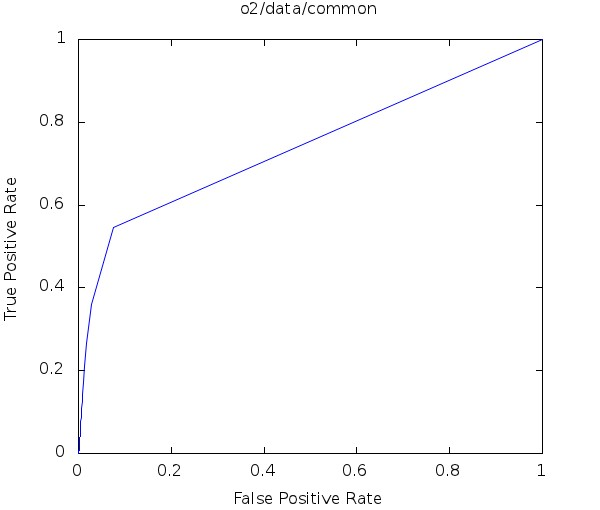
\includegraphics[width=0.4\textwidth]{../roc/o2/fig/common.jpg}
}
\subfigure[PR: EV=High 3]{
\label{fig:roc_selected_pr_high}
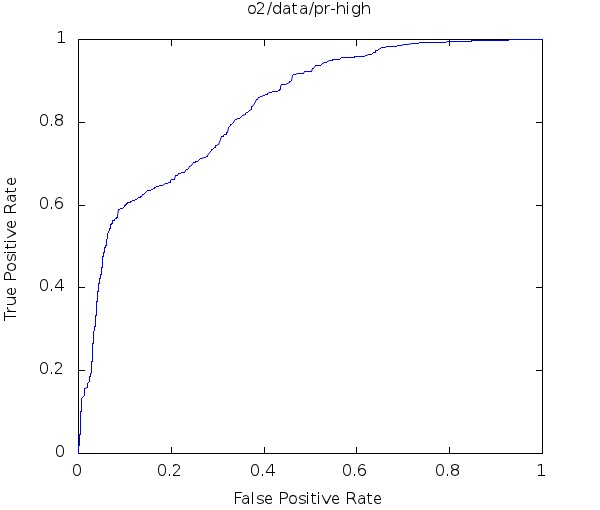
\includegraphics[width=0.4\textwidth]{../roc/o2/fig/pr_high.jpg}
}
\caption{Selected ROC Curves}
\label{fig:roc_selected}
\end{figure}

Our observations of those ROC curves are listed below:
\begin{enumerate}
	\item All ROC curves blend above the line TPR=FPR. This means, 
	those proximity measures can reflect similarity between observer
	and other nodes. They are absolutely better than random guess. 
	\item All ROC curves have a switching point, which locates 
	at the low FPR region. Before this point, the curve increases 
	sharply, after this point, the tangent of the curve decreases.
	This means, those proximity measures alone can be used to detect 
	community with high precision when $T$ is large. They can 
	hardly distinguish nodes with low proximity measure. 
	\item Among all the 9 curves, PageRank with escape vector set to 
	3 highest degree nodes performs the best. See, fig(\ref{fig:roc_selected_pr_high}). 
	The area under this curve is the largest. This proves 
	the efficacy of our proposed semi-supervised version of PPR. 
	The introduction of high influential nodes in the same community
	can help to detect other members. 
\end{enumerate}


\section{Model Training and Testing}

%=====================data=====

%observer 2, full nodes. MLP, default. 
%=== Detailed Accuracy By Class ===
%
%               TP Rate   FP Rate   Precision   Recall  F-Measure   ROC Area  Class
%                 0.383     0.031      0.599     0.383     0.468      0.746    1
%                 0.969     0.617      0.929     0.969     0.949      0.746    0
%Weighted Avg.    0.906     0.554      0.894     0.906     0.897      0.746
%
%=== Confusion Matrix ===
%
%     a     b   <-- classified as
%  1812  2915 |     a = 1
%  1212 38180 |     b = 0

%observer 2, cut degree leq1. MLP, default. 
%
%=== Detailed Accuracy By Class ===
%
%               TP Rate   FP Rate   Precision   Recall  F-Measure   ROC Area  Class
%                 0.534     0.202      0.699     0.534     0.606      0.72     1
%                 0.798     0.466      0.661     0.798     0.723      0.72     0
%Weighted Avg.    0.675     0.342      0.679     0.675     0.668      0.72 
%
%=== Confusion Matrix ===
%
%    a    b   <-- classified as
% 1382 1205 |    a = 1
%  595 2348 |    b = 0
%  %

%observer 2, cut degree leq2. MLP, default.
%=== Detailed Accuracy By Class ===
%
%               TP Rate   FP Rate   Precision   Recall  F-Measure   ROC Area  Class
%                 0.987     0.916      0.639     0.987     0.776      0.69     1
%                 0.084     0.013      0.793     0.084     0.151      0.69     0
%Weighted Avg.    0.645     0.575      0.697     0.645     0.54       0.69 
%
%=== Confusion Matrix ===
%
%    a    b   <-- classified as
% 1706   23 |    a = 1
%  963   88 |    b = 0


%observer 2, only level 1. MLP, default
%=== Detailed Accuracy By Class ===
%
%               TP Rate   FP Rate   Precision   Recall  F-Measure   ROC Area  Class
%                 0.685     0.173      0.813     0.685     0.744      0.801    1
%                 0.827     0.315      0.704     0.827     0.761      0.801    0
%Weighted Avg.    0.752     0.241      0.761     0.752     0.752      0.801
%
%=== Confusion Matrix ===
%
%  a  b   <-- classified as
% 74 34 |  a = 1
% 17 81 |  b = 0

%==============================data end ================

From the above analysis, we notice that although those 
proximity measures reflect community information to some degree, 
none of them can provide perfect ROC alone. In this section, 
we train Multi-Layer Perceptron using weka\cite{weka}, aiming at
combining those features and outputing better results. 

\subsection{MLP with Full Topology}

Our first experiment is to train an MLP with full topology. 
Let observer 2 be an example, the confusion matrix on testing 
data is shown in table(\ref{tbl:cm_o2_full}). 

\begin{table}[htb]
	\centering
	\caption{Confusion Matrix: MLP, Observer2, Full Topology}
	\label{tbl:cm_o2_full}
	\begin{tabular}{cc|c}
	\hline
a & b & \textbf{$\leftarrow$ classified as}\\	
	\hline
1812 &  2915 &    $a = 1$ \\
1212 & 38180 &    $b = 0$\\
	\hline
	\end{tabular}
\end{table}

The precision is 0.599 and recall is 0.383. The overall accuracy 
is 0.906. Although the overall accuracy is very high, we can 
conclude that this classification is of low application value. 
The True Negative population is very large, which means our trained 
MLP tends to classify nodes into class 0. 

One of our targeted use of the predicted labels can be friend 
recommendation. It's nonsense to recommend a lot of friends 
at a time. So our application is not sensitive to recall rate. 
Thus we work towards higher precision in the successive experiments, 
and at the same time avoid making the predication trivial. 

\subsection{MLP without Degree 1 Nodes}

\question

According to our previous statistics, large amount of nodes
are of degree one. This doesn't necessarily mean the real 
degree, but means the degree within our observation. 
The 2-hop topology is so limited that we see many leaf nodes. 

\begin{figure}[htb]
	\centering
	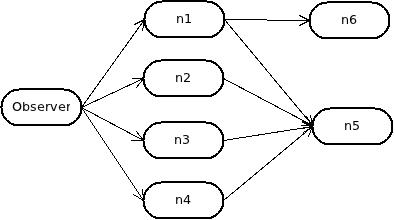
\includegraphics[width=0.5\linewidth]{fig/illustration_2hop_level2.jpg}
	\caption{Illustration of Two Levels}
	\label{fig:illu_l2}
\end{figure}

Fig(\ref{fig:illu_l2}) illustrates one part of the 2-hop 
topology. The real friend relationship is bidirectional. 
The arrows in the illustration just represents the direction 
of our crawler. Nodes n5 and n6 stand for two typical situations 
of those level 2 nodes. It's very probable that n6 with single link 
from a level 1 node is not in the observer's community. 
On the contrary, n5, which many level 1 nodes point to is very likely
to be in the same community as observer. 

Nodes like n6 will bring up priori probability of class 0 as shown in 
the previous experiment. We eliminate all nodes with degree 1, and 
run the training stage again. Result confusion matrix is shown 
in table(\ref{tbl:cm_o2_d1}). 

\begin{table}[htb]
	\centering
	\caption{Confusion Matrix: MLP, Observer2, without Degree 1}
	\label{tbl:cm_o2_d1}
	\begin{tabular}{cc|c}
	\hline
a & b & \textbf{$\leftarrow$ classified as}\\	
	\hline
 1382 &1205 &    $a = 1$\\
  595 &2348 &    $b = 0$\\
	\hline
	\end{tabular}
\end{table}

The precision is now 0.699 and recall is  0.534. 
Both metrics are improved, while the overall accuracy 
degrades to 0.675. Bearing our potential application in mind, 
this result is better, which means if we target 10 nodes 
from the predicted positive class, we may have a chance
of 70\% to hit observer's community. 

\subsection{MLP without Degree 2}

Take the last experiment further, it's rational to 
think whether eliminating more nodes can help. 

We train the same model after eliminating degree 2 nodes. 
The result confusion matrix is shown in table().

\begin{table}[htb]
	\centering
	\caption{Confusion Matrix: MLP, Observer2, without Degree 2}
	\label{tbl:cm_o2_d2}
	\begin{tabular}{cc|c}
	\hline
a & b & \textbf{$\leftarrow$ classified as}\\	
	\hline
 1706 &23 &    $a = 1$\\
  963 &88 &    $b = 0$\\
	\hline
	\end{tabular}
\end{table}

The precision is now 0.639 and recall is 0.987. 
Though we get a very good recall rate, the precision 
is lowered. Looking into the confusion matrix, 
we find this classification becomes \textbf{trivial}. 
It tends to predict class 1. Even a naive guess 
that classifies all nodes into class 1 can reach 
the precision of 0.62194 and recall 1.0. 

With more lower degree nodes being eliminated, 
we may think this problem becomes more significant. 
Since the priori probability of class 1 increases, 
the naive guess precision can increase by keeping 
a 100\% recall. 

\subsection{MLP with Only Level 1 Nodes}

If we limit our mining scope to only level 1 nodes, 
the application can not be friend recommendation, since 
they have alreay established one link with observer. 
Nevertheless, taking a look at the result is of great interest. 
table(\ref{tbl:cm_o2_l1}) shows the result confusion matrix. 

\begin{table}[htb]
	\centering
	\caption{Confusion Matrix: MLP, Observer2, Only Level 1 Nodes}
	\label{tbl:cm_o2_l1}
	\begin{tabular}{cc|c}
	\hline
a & b & \textbf{$\leftarrow$ classified as}\\	
	\hline
 74 &34 &    $a = 1$\\
  17 &81 &    $b = 0$\\
	\hline
	\end{tabular}
\end{table}

The precision is 0.813, and the recall is 0.685. 
If we aim at the "community" defined as a group 
of people sharing the same interest, rather than 
those institutions, this result suggests targeted 
advertisement can be performed effeciently. 


\section{Conclusion}

This paper shows 2-hop link topology contains some information, 
though it is limited. We highlight the following 
observations from the study:
\begin{enumerate}
	\item 
\end{enumerate}

\section{Future Work}

\subsection{More Metrics}

As is in our proposal \cite{hu2011-cd2hop}, there are other metrics
we want to try. Due to project time and report space, we only name 
a few in this section:
\begin{itemize}
	\item Katz Score:
			\begin{equation}
				Katz(i,j)=\sum_{l=1}^{\infty}{\beta^lA^l(i,j)}
			\end{equation}
			The matrix series results in 
			\begin{equation}
				Katz = (I-\beta A)^{-1} - I
			\end{equation}
			By tuning $\beta$, this score can measure number of paths between 
			two nodes, with preferred length range. 
	\item Simrank:
			\begin{equation}
				s(a,b)=\frac{\gamma}{|I(a)||I(b)|}
				\sum_{i \in I(a), j \in I(b)} s(i,j)
			\end{equation}
			This metric measures the expectation of $\gamma^l$, where $l$ equals 
			the time when two random walkers start from $a$ and $b$ meet. By proper 
			matrix construction, Simrank can be solved as an eigenvalue problem. 
\end{itemize}
For more information, interested readers are recommended to \cite{aggarwal2011social}. 

\subsection{Broader Data Source}

The links used in this study is mere static topology. 
With 2-hop limit, the information can be extracted 
is not abundant. In terms of data source, we propose 
two promising directions:
\begin{enumerate}
	\item Dynamic link information. "renren.com" is a very 
	dense graph. However, many edges are not effetive in the sense
	that little information flow through them. We can 
	build links using user interactions like status forwarding, 
	blog reply, etc. 
	\item Content based prediction. Note that links can only capture
	static topology or dynamic interaction, but not content. Nodes in a 
	well-defined community share similar content with very high 
	probability. Combining topology and content may be a promising 
	direction. 
\end{enumerate}

Similar thoughts have been proposed in many related literature, to name 
a few\cite{boccaletti2006complex,aggarwal2011social}. 

\subsection{Fine-grained Variations of PR}

The variations of PageRank have great potential. We
shortlist a few possible directions:
\begin{enumerate}
	\item What's the most appropriate transition ratio $\alpha$. 
	\item How many influential nodes should be introduced 
	in the semi-supervised version of PPR, considering
	both cost and accuracy. 
\end{enumerate}

\subsection{Quality Functions}

After we label the community of all nodes, we can calculate some quality 
functions to indicate how well the community is detected. Different researchers
have different preference of quality functions, to name a few:
	\begin{itemize}
		\item Normalized cut:
		\begin{equation}
			Ncut(S)=\frac{\sum_{i \in S, j \in \overline{S}}{A(i,j)}}
			{\sum_{i \in S}{d(i)}}
			+ \frac{\sum_{i \in S, j \in \overline{S}}{A(i,j)}}
			{\sum_{j \in \overline{S}}{d(j)}}					
			\label{eq:ncut}	
		\end{equation}
		where $S$ is the set of one community, 
		and $d(.)$ is the digree of a node, which is defined as 
		$d(i)=\sum_j{A_{ij}}$.
		
		The smaller the value, the better community detection quality. 
		Two numerators measure the number of inter community links, 
		and the value is normalized by the number of intra community links. 
		\item Conductance:
		\begin{equation}
			Conductance(S)=\frac{\sum_{i \in S, j \in \overline{S}}{A(i,j)}}
			{\min \{ \sum_{i \in S}{d(i)}, \sum_{j \in \overline{S}}{d(j)}\}}	
			\label{eq:conductance}			
		\end{equation}
		This quality function is positive related with eqn(\ref{eq:ncut}). 
		When community sizes are highly skewed, conductance may provide 
		better evaluation. 
		\item Modularity:
		\begin{equation}
			Q=\sum_{i=1}^{K}{\left[ 
			\frac{A(V_i,V_i)}{m} 
			-\left( \frac{d(V_i)}{2m}\right)^2
			\right]}
			\label{eq:modularity}
		\end{equation}
		where 
		\begin{equation}
			A(V_i,V_j)= \sum_{u \in V_i,v \in V_j}{A_{uv}}
		\end{equation}
		and 
		\begin{equation}
			d(V_i)=\sum_{u \in V_i}{d_u}
		\end{equation}
		$K$ is the number of communities, which is 2 in our case
		(we only distinguish whether the node is in the same community
		with observer or not).
		
		The rationale behind modularity is the comparison with a random 
		graph. The father resultant community is from a random graph, 
		the better the quality. "One of the advantages of modularity is 
		that it is independent of the number of communities the graph is
		divided into"\cite{aggarwal2011social}. 
	\end{itemize}
	
	Those quality functions are popular among different research 
	groups. They also capture different characteristics of graphs. 
	In this project, we'll check if these global metric can 
	be used to evaluate our extreme local case. 

\section*{Acknowledgements}

The authors would like to thank the following people for their contribution of 
personal data: 
Bo WANG, Hongshu LIAO, Huan CHEN, Shouxi LUO, 
Xiaoyu LUO, Xinyue ZHENG, Yan WANG, Yi LUO. 
The authors appreciate brain storm discussion with professor Wing Lau 
and Deyi Sun. 
The authors would like to thank course instructors and TAs of CSCI5180. 


%begin================bibliography======================

%this seems impossible to merge automatically
%at the same time, I don't want to construct .bib databse
%for all these temporary entries. 
%
%my solution is to extract bibentries and paste them in 
%the following {thebibliography} section
%
%
%%\bibliographystyle{plain}
%%\bibliography{mylibrary}

%%%%GENBIBSTRING%%%%

\begin{thebibliography}{99}

%cut and paste section 
%generate by 'make bib' from my bib database
\bibitem{hu2011-cd2hop}
Hu~Pili and Li~Yichao.
\newblock Community detection on 2-hop topology.
\newblock GitHub, https://github.com/Czlyc/2C-Web-Research, 12 2011.
\newblock course project of CUHK/CSCI5180.

\bibitem{aggarwal2011social}
C.C. Aggarwal.
\newblock {\em Social network data analytics}.
\newblock Springer-Verlag New York Inc, 2011.

\bibitem{breslau1999web-zipf}
L.~Breslau, P.~Cao, L.~Fan, G.~Phillips, and S.~Shenker.
\newblock Web caching and zipf-like distributions: Evidence and implications.
\newblock In {\em INFOCOM'99. Eighteenth Annual Joint Conference of the IEEE
  Computer and Communications Societies. Proceedings. IEEE}, volume~1, pages
  126--134. IEEE, 1999.

\bibitem{boccaletti2006complex}
S.~Boccaletti, V.~Latora, Y.~Moreno, M.~Chavez, and D.U. Hwang.
\newblock Complex networks: Structure and dynamics.
\newblock {\em Physics reports}, 424(4-5):175--308, 2006.


%temporary section
	\bibitem{csci5180_lecture} CSCI5180, Data Mining Lecture Notes, 
		\url{http://www.cse.cuhk.edu.hk/~lwchan/teaching/csc5180.html}
	\bibitem{csci5180_tutorial} CSCI5180, Data Mining Tutorial Notes. 
		(available in Moodle. Please contact the teacher/TA if you have 
		interest)
	\bibitem{wiki_roc} Receiver Operating Characteristics, 
		\url{http://en.wikipedia.org/wiki/Receiver_operating_characteristic}
	\bibitem{weka} Weka, 
		\url{http://www.cs.waikato.ac.nz/ml/weka/index.html}
	\bibitem{wiki_iso_graph} Wikipedia, Isomorphic Graph, 
		\url{http://en.wikipedia.org/wiki/Graph_isomorphism}
	\bibitem{nodexl} NodeXL, 
		\url{http://nodexl.codeplex.com/}
\end{thebibliography}

%end================bibliography======================


\section*{Appendix}

\subsection*{ROC Algorithm}

This algorithm runs in $O(n)$ time, where 
$n$ is the number of data points. This algorithm 
is applicable where TP and FP is monotonic w.r.t 
the $T$ threshold. 

\begin{Verbatim}
FUNCTION (Nodes[])
	calculate CountPositive, CountNegative
	T = -infinite
	TP = CountPositive
	FP = CountNegative
	sort Nodes according to proximity measure. 
	FOR i = 0 ; i < CountTotal ; i ++ 
		IF T < Nodes(i).proximity THEN
			OUTPUT T, TP / CountPositive, FP / CountNegative
		END IF
		T = Nodes(i).proximity
		IF Nodes(i).label == 1 THEN
			TP -- 
		ELSE
			FP --
		END IF
	END FOR
END FUNCTION
\end{Verbatim}

\subsection*{ROC Curve of Observer 2}

ROC curves of 9 features are shown in fig(\ref{fig:roc_sub_all}).
It's obvious that PageRank with escape vector using 3 highest 
degree nodes and without super node performs the best alone, 
see fig(\ref{fig:roc_sub_pr_high}). 

\begin{figure}[htb]
    \label{fig:subfigures}
    \begin{center}
%
        \subfigure[Common Neighbour]{%
            \label{fig:roc_sub_common}
            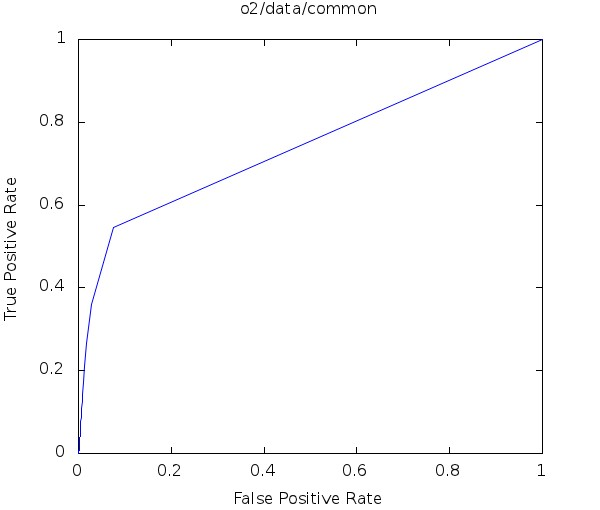
\includegraphics[width=0.3\textwidth]{../roc/o2/fig/common.jpg}
        }%
        \subfigure[Ademic/Adar]{%
           \label{fig:roc_sub_adamic}
           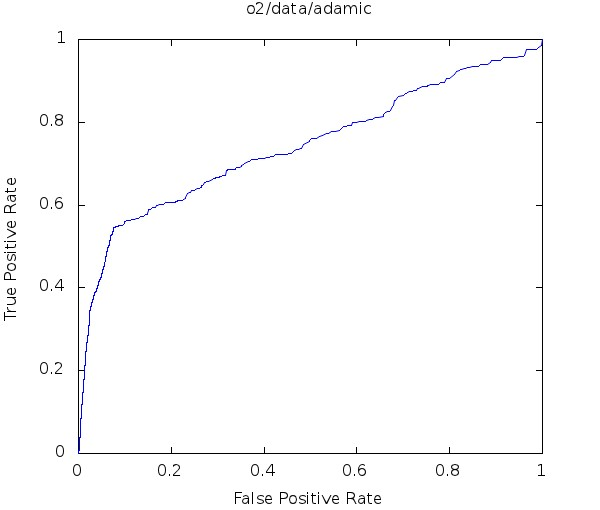
\includegraphics[width=0.3\textwidth]{../roc/o2/fig/adamic.jpg}
        }
        \subfigure[Jaccard's]{%
            \label{fig:roc_sub_jacc}
            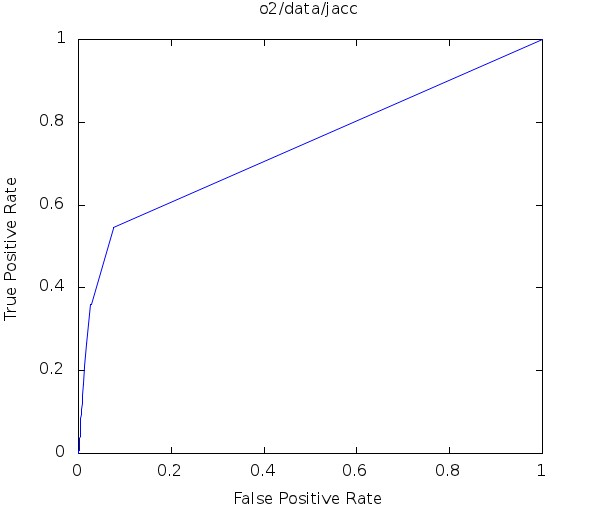
\includegraphics[width=0.3\textwidth]{../roc/o2/fig/jacc.jpg}
        }\\%

        \subfigure[PR:EV=All 1's]{%
            \label{fig:roc_sub_pr_all1}
            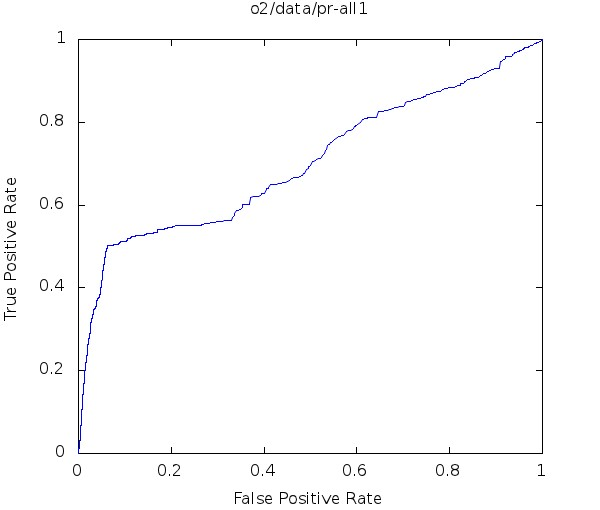
\includegraphics[width=0.3\textwidth]{../roc/o2/fig/pr_all1.jpg}
        }%
        \subfigure[PR:EV=High 3]{%
           \label{fig:roc_sub_pr_high}
           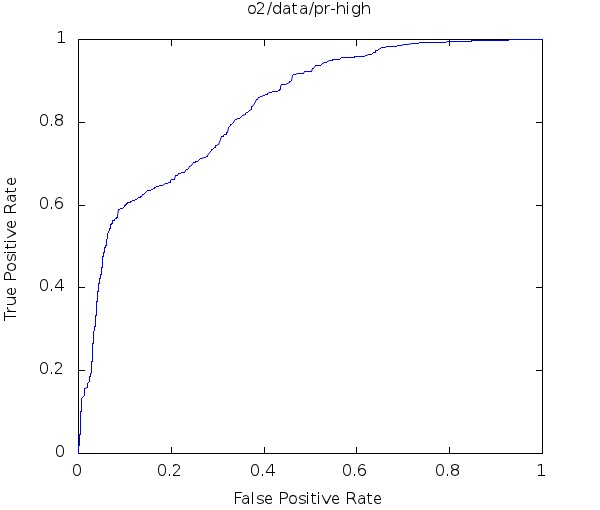
\includegraphics[width=0.3\textwidth]{../roc/o2/fig/pr_high.jpg}
        }
        \subfigure[PR:EV=Root]{%
            \label{fig:roc_sub_pr_root}
            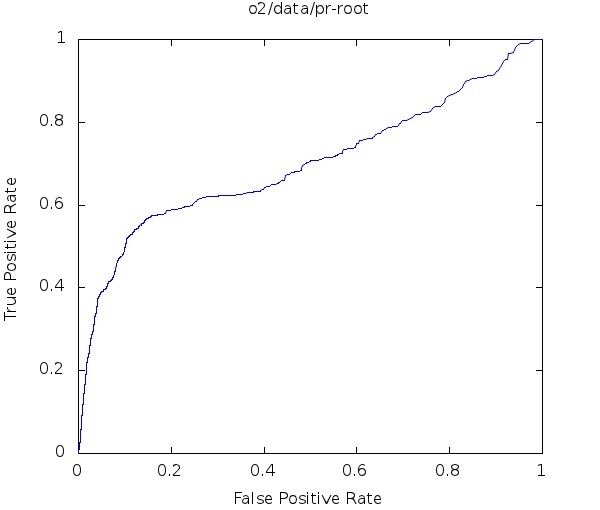
\includegraphics[width=0.3\textwidth]{../roc/o2/fig/pr_root.jpg}
        }\\%
        
        \subfigure[PR:EV=All 1's(+SN)]{%
            \label{fig:roc_sub_pr_all1_super}
            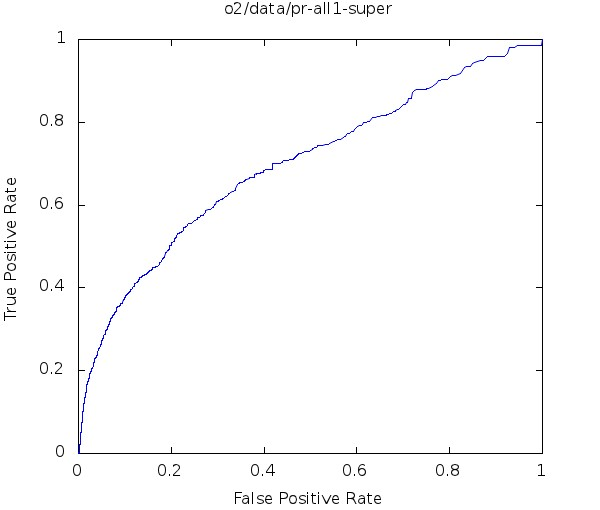
\includegraphics[width=0.3\textwidth]{../roc/o2/fig/pr_all1_super.jpg}
        }%
        \subfigure[PR:EV=High 3 (+SN)]{%
           \label{fig:roc_sub_pr_high_super}
           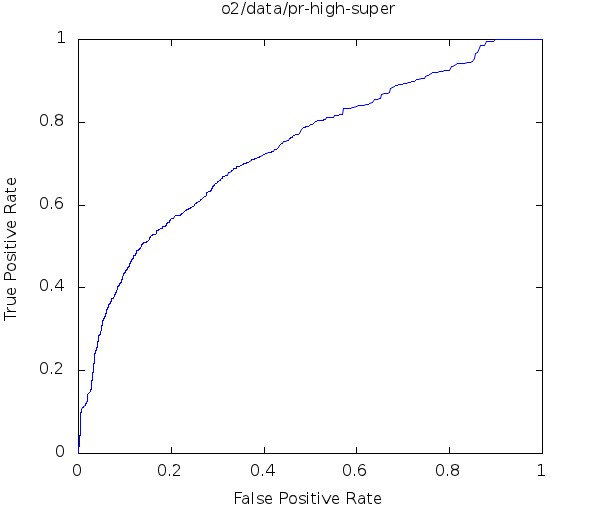
\includegraphics[width=0.3\textwidth]{../roc/o2/fig/pr_high_super.jpg}
        }
        \subfigure[PR:EV=Root(+SN)]{%
            \label{fig:roc_sub_pr_root_super}
            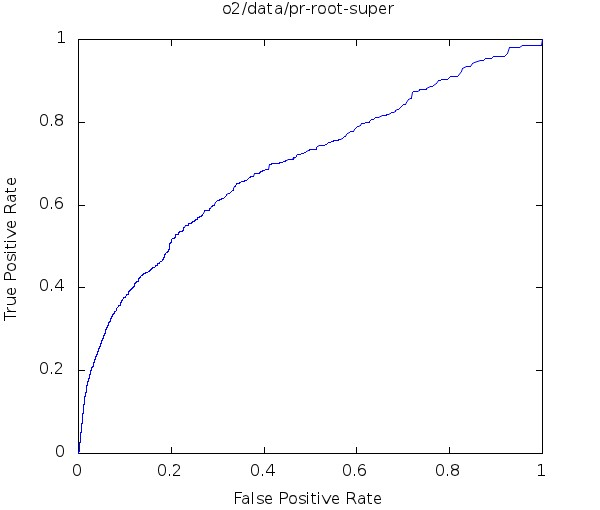
\includegraphics[width=0.3\textwidth]{../roc/o2/fig/pr_root_super.jpg}
        }\\%
%
    \end{center}
    \caption{%
        ROC Curve of 9 Features
     }%
     \label{fig:roc_sub_all}
\end{figure}


 

\section*{Declaration}

Meta tools like PageRank, Adamic/Adar, etc, are learned from the book
\textit{Social Network Data Analytics}. For original sources of these 
algorithms, please refer to the bibliography pages of that book.

The analysis/adaptation/extension/application of these tools and 
the use in community detection on 2-hop topology mentioned 
in this document is originality. Please refer to our open source 
repository for citation issues.

\textbf{\textit{
The data in our project repository is limited to research use only. 
The authors of this paper own the transformed version. You are welcome
to use them in your study but remember to make a notification to the 
authors first. Our contact information is given in the project 'README' file. }}

\end{document}
